% Pixelkatze – Programmarchitektur (eine Seite A4)
% Kompilieren mit XeLaTeX oder LuaLaTeX, z. B.:  tectonic pixelkatze-architektur.tex  ·  xelatex pixelkatze-architektur.tex
\documentclass{article}

\usepackage[a4paper, left=20pt, right=20pt, top=67pt, bottom=22pt, nohead, nofoot]{geometry}
\usepackage{fontspec}
\usepackage{xcolor}
\usepackage{graphicx}
\usepackage{tikz}
\usetikzlibrary{arrows.meta, calc}
\usepackage{tabularx}
\usepackage{colortbl}
\usepackage{enumitem}
\usepackage{amssymb}
\usepackage{ragged2e}

% ---------- Schriften ----------
% Freie Schriften mit fest benannten Schnitten – laufen auf jedem System (auch Overleaf)
\setmainfont{texgyreheros}[Extension=.otf, UprightFont=*-regular, BoldFont=*-bold,
  ItalicFont=*-italic, BoldItalicFont=*-bolditalic]
\setmonofont{DejaVuSansMono}[Extension=.ttf, BoldFont=*-Bold, Scale=0.9]
\newfontfamily\titlefont{texgyreheros}[Extension=.otf, UprightFont=*-bold]

% ---------- Farben (wie die Katze) ----------
\definecolor{ink}{HTML}{2B1D16}
\definecolor{muted}{HTML}{6B5A4F}
\definecolor{orange}{HTML}{F2A14B}
\definecolor{orangedark}{HTML}{C96F2E}
\definecolor{cream}{HTML}{FFF7EC}
\definecolor{line}{HTML}{E8D6C2}
\definecolor{rowline}{HTML}{F1E6DA}
\definecolor{blue}{HTML}{3E6FA8}
\definecolor{green}{HTML}{4F8A3C}
\definecolor{red}{HTML}{C0392B}
\definecolor{codebg}{HTML}{F6EEE4}
\definecolor{sysfill}{HTML}{EEF3F9}
\definecolor{sysdraw}{HTML}{9DB6D3}
\definecolor{boxdraw}{HTML}{C9B29A}
\definecolor{corefill}{HTML}{FFF1DF}
\definecolor{arrow}{HTML}{8B7B70}
\definecolor{tagin}{HTML}{FBE7DA}
\definecolor{tagcl}{HTML}{E6EEF8}
\definecolor{tagro}{HTML}{E7F1E2}
\definecolor{dock}{HTML}{5B4A52}
\definecolor{dockdark}{HTML}{4B3D44}

% ---------- Grundeinstellungen ----------
\renewcommand\normalsize{\fontsize{6.95pt}{10.1pt}\selectfont}
\pagestyle{empty}
\setlength\parindent{0pt}
\setlength\parskip{2pt}
\setlength\tabcolsep{2pt}
\color{ink}
\RaggedRight

% ---------- Bausteine ----------
\newcommand\code[1]{{\setlength\fboxsep{0.7pt}\colorbox{codebg}{\ttfamily\fontsize{6.1pt}{8pt}\selectfont #1}}}
\newcommand\mono[1]{{\ttfamily\fontsize{6.1pt}{8pt}\selectfont\color{blue}#1}}
\newcommand\sect[1]{%
  \par\vspace{1pt}%
  {\color{orangedark}\bfseries\fontsize{7.8pt}{9pt}\selectfont\addfontfeature{LetterSpace=8}\MakeUppercase{#1}}\par
  \vspace{-3pt}{\color{orange}\rule{\linewidth}{1.2pt}}\par\vspace{1pt}}
\newcommand\chip[1]{\tikz[baseline=(c.base)]\node(c)[draw=line, fill=cream, rounded corners=4.5pt,
  inner xsep=4.5pt, inner ysep=1.6pt, font=\fontsize{6.2pt}{7pt}\selectfont]{#1};}
\newcommand\hl[1]{{\bfseries\color{orangedark}#1}}
\newcommand\tagx[2][codebg]{\tikz[baseline=(t.base)]\node(t)[fill=#1, rounded corners=1.2pt, inner xsep=1.6pt,
  inner ysep=0.9pt, font=\ttfamily\fontsize{5.9pt}{7pt}\selectfont]{#2};\hspace{1.2pt}\allowbreak}
\newcommand\stepnum[1]{\tikz[baseline=-0.62ex]\node[circle, fill=orange, inner sep=0pt, minimum size=8.6pt,
  text=white, font=\bfseries\fontsize{5.6pt}{6pt}\selectfont]{#1};}
\newcommand\callout[1]{\par\vspace{2pt}{\setlength\fboxsep{0pt}\noindent
  \tikz\node[fill=cream, inner xsep=4pt, inner ysep=2.5pt, text width=\linewidth-8pt, align=left,
  path picture={\fill[orange] (path picture bounding box.north west) rectangle ([xshift=2.2pt]path picture bounding box.south west);}]{#1};}\par}
\newcommand\arr{$\rightarrow$}

\setlist{nosep, leftmargin=10pt}
\newlist{steps}{enumerate}{1}
\setlist[steps]{label=\protect\stepnum{\arabic*}, leftmargin=12pt, labelsep=3pt, itemsep=1.2pt, topsep=0pt}
\newlist{order}{enumerate}{1}
\setlist[order]{label=\arabic*., leftmargin=10pt, labelsep=3pt, itemsep=0.8pt, topsep=1pt}

% Tabelle mit hellen Trennlinien
\newcommand\kvrow[2]{\mono{#1} & #2 \\ \arrayrulecolor{rowline}\hline}

\begin{document}

% ================= Kopf und Fuß (absolut positioniert) =================
\begin{tikzpicture}[remember picture, overlay]
  \coordinate (nw) at (current page.north west);
  \fill[white] (current page.south west) rectangle (current page.north east);
  \fill[ink] (nw) rectangle ([xshift=595pt, yshift=-62pt]nw);
  \foreach \i in {0,...,13} {
    \fill[dock]     ([xshift=\i*44pt, yshift=-62pt]nw) rectangle ([xshift=\i*44pt+22pt, yshift=-58pt]nw);
    \fill[dockdark] ([xshift=\i*44pt+22pt, yshift=-62pt]nw) rectangle ([xshift=\i*44pt+44pt, yshift=-58pt]nw);
  }
  \node[anchor=base west, inner sep=0, text=cream] at ([xshift=20pt, yshift=-35pt]nw)
    {\titlefont\fontsize{19pt}{20pt}\selectfont Pixel\textcolor{orange}{katze} – Programmarchitektur};
  \node[anchor=base west, inner sep=0, text=cream!85] at ([xshift=20pt, yshift=-49pt]nw)
    {\fontsize{7.4pt}{9pt}\selectfont Aufbau, Technik und Ablauf der Dock-Katze für macOS · Version 5.2};
  \node[anchor=south east, inner sep=0] at ([xshift=575pt, yshift=-58pt]nw) {%
    
\includegraphics[height=25pt]{img/stand-orange.png}\hspace{7pt}%
    
\includegraphics[height=19pt]{img/stretch.png}\hspace{7pt}%
    
\includegraphics[height=25pt]{img/stand-gray.png}\hspace{7pt}%
    
\includegraphics[height=19pt]{img/sleep.png}\hspace{7pt}%
    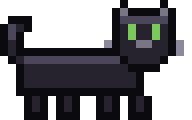
\includegraphics[height=25pt]{img/stand-black.png}};
  % Fußzeile
  \draw[line] ([xshift=20pt, yshift=18pt]current page.south west) -- ([xshift=-20pt, yshift=18pt]current page.south east);
  \node[anchor=base west, inner sep=0, text=muted, font=\fontsize{6.1pt}{7pt}\selectfont]
    at ([xshift=20pt, yshift=9pt]current page.south west) {Quellcode: github.com/TheesBudde/pixelkatze · Version 5.2};
  \node[anchor=base east, inner sep=0, text=muted, font=\fontsize{6.1pt}{7pt}\selectfont]
    at ([xshift=-20pt, yshift=9pt]current page.south east) {Katzenlaute: „Cat Purr \& Meow“, Kerzoven (opengameart.org), CC0};
\end{tikzpicture}%

% ================= Technik-Leiste =================
\noindent\chip{\hl{Swift 5} (Compiler 6.3)}\hfill
\chip{\hl{AppKit} – Fenster, Menü}\hfill
\chip{\hl{Core Graphics} – Pixel, Fenster}\hfill
\chip{\hl{NSSound} – Töne}\hfill
\chip{keine Fremdbibliotheken}\hfill
\chip{7 Dateien · $\approx$ 3.000 Zeilen}

\vspace{5pt}

% ================= Architekturdiagramm =================
\noindent\begin{tikzpicture}[x=1pt, y=-1pt,
    sys/.style={draw=sysdraw, fill=sysfill, rounded corners=4pt, line width=0.6pt},
    box/.style={draw=boxdraw, fill=white, rounded corners=5pt, line width=0.6pt},
    core/.style={draw=orange, fill=corefill, rounded corners=5pt, line width=1.2pt},
    t1/.style={anchor=base west, inner sep=0, font=\bfseries\fontsize{8pt}{9pt}\selectfont, text=ink},
    t2/.style={anchor=base west, inner sep=0, font=\fontsize{6.6pt}{8pt}\selectfont, text=muted},
    fn/.style={anchor=base west, inner sep=0, font=\ttfamily\bfseries\fontsize{6.1pt}{7pt}\selectfont, text=blue},
    lb/.style={anchor=base west, inner sep=0, font=\itshape\fontsize{6.2pt}{7pt}\selectfont, text=arrow},
    ar/.style={draw=arrow, line width=0.7pt, -{Stealth[length=3.6pt, width=3.2pt]}}]
  % Rahmen mit Überschrift
  \shade[top color=white, bottom color=cream, rounded corners=6pt, draw=line] (-8,-22) rectangle (547,228);
  \node[anchor=base west, inner sep=0] at (0,-11)
    {\color{orangedark}\bfseries\fontsize{7.8pt}{9pt}\selectfont\addfontfeature{LetterSpace=8}AUFBAU – WER REDET MIT WEM?};
  \draw[orange, line width=1.2pt] (0,-7) -- (539,-7);

  % macOS
  \node[lb, font=\bfseries\fontsize{6.2pt}{7pt}\selectfont, text=blue] at (0,7) {macOS};
  \foreach \x/\a/\b in {0/Menüleiste/NSStatusItem, 110/Dock-Oberkante/NSScreen.visibleFrame,
                        220/Offene Fenster/CGWindowList…, 330/Maus/NSEvent.mouseLocation, 440/Lautsprecher/NSSound} {
    \draw[sys] (\x,12) rectangle ++(98.5,32);
    \node[t1] at (\x+6,25) {\a};
    \node[fn] at (\x+6,37) {\b};
  }

  % AppDelegate
  \draw[box] (0,66) rectangle (150,124);
  \node[t1] at (7,79) {AppDelegate}; \node[fn] at (82,79) {AppDelegate.swift};
  \node[t2] at (7,91)  {Menü aufbauen \& aktualisieren,};
  \node[t2] at (7,100) {Einstellungen speichern (UserDefaults),};
  \node[t2] at (7,109) {Eingabedialog „Eigene Zeit …“,};
  \node[t2] at (7,118) {Restzeit neben dem Symbol anzeigen};

  % CatController
  \draw[core] (172,66) rectangle (539,124);
  \node[t1] at (179,79) {CatController – die Steuerzentrale}; \node[fn] at (470,79) {Controller.swift};
  \node[t2] at (179,91)  {• Takt: Timer, 30-mal pro Sekunde – bewegt alles und zeichnet neu};
  \node[t2] at (179,100) {• Pomodoro (25/5 Min.), eigener Timer, Pausen-Erinnerung (45–55 Min.)};
  \node[t2] at (179,109) {• Fensterkanten zum Klettern berechnen · Streicheln erkennen · Napf \& Wollknäuel (Physik)};
  \node[t2] at (179,118) {• entscheidet, wann miaut wird, und blendet die Katze im Streifzug aus};

  % Ebene 3
  \draw[core] (172,146) rectangle (350,186);
  \node[t1] at (179,159) {CatBrain – Verhalten}; \node[fn] at (306,159) {Cat.swift};
  \node[t2] at (179,170) {Zustandsautomat mit 25 Phasen, Modi,};
  \node[t2] at (179,179) {Ziele, Klettern, Streifzug, Tageszeit};

  \draw[box] (361,146) rectangle (539,186);
  \node[t1] at (368,159) {Darstellung}; \node[fn] at (448,159) {CatView · PropWindow};
  \node[t2] at (368,170) {randlose, durchsichtige Fenster (NSPanel),};
  \node[t2] at (368,179) {Pixel zeichnen, Klicks nur auf Katzenpixeln};

  \draw[box] (0,146) rectangle (150,186);
  \node[t1] at (7,159) {Start}; \node[fn] at (36,159) {main.swift · Export.swift};
  \node[t2] at (7,170) {startet die App (ohne Dock-Symbol) –};
  \node[t2] at (7,179) {oder erzeugt App-Symbol \& Vorschau};

  % Ebene 4
  \draw[box] (172,200) rectangle (350,222);
  \node[t1] at (179,214) {Frames \& Coat}; \node[t2] at (243,214) {Pixelraster + Fellfarben}; \node[fn] at (318,214) {Sprites};
  \draw[box] (361,200) rectangle (539,222);
  \node[t1] at (368,214) {Meow}; \node[t2] at (394,214) {3 echte Katzenaufnahmen (CC0)}; \node[fn] at (510,214) {Sound};
  \draw[box] (0,200) rectangle (150,222);
  \node[t1] at (7,214) {build.sh · release.sh}; \node[t2] at (93,214) {\arr\ Pixelkatze.app};

  % Pfeile
  \draw[ar] (49,44) -- (49,64);   \node[lb] at (53,57) {Menüklick};
  \draw[ar] (150,95) -- (170,95);
  \draw[ar] (159,44) -- (230,64);
  \draw[ar] (269,44) -- (290,64); \node[lb] at (292,56) {Fensterliste};
  \draw[ar] (379,44) -- (380,64); \node[lb] at (384,57) {Maus};
  \draw[ar] (489,64) -- (489,46); \node[lb] at (493,57) {Miau};
  \draw[ar] (240,124) -- (240,144); \node[lb, anchor=base east] at (236,137) {update(dt), Ereignisse};
  \draw[ar] (280,144) -- (280,126); \node[lb] at (284,137) {Position x/y, look};
  \draw[ar] (440,124) -- (440,144); \node[lb, anchor=base east] at (436,137) {Fenster setzen, zeichnen};
  \draw[ar] (505,144) -- (505,126); \node[lb] at (509,137) {Klick};
  \draw[ar] (261,186) -- (261,198);
  \draw[ar] (450,186) -- (450,198);
  \draw[ar, dash pattern=on 2pt off 2pt] (75,124) -- (75,144);
  \draw[ar, dash pattern=on 2pt off 2pt] (75,186) -- (75,198);
\end{tikzpicture}

\vspace{4pt}

% ================= Drei Spalten (als ein Block gesetzt) =================
\newsavebox\spalten
\sbox\spalten{%
%-------------------------------- Spalte 1
\begin{minipage}[t]{172pt}
\sect{Dateien}
\renewcommand\arraystretch{1.05}
\begin{tabularx}{\linewidth}{@{}l@{\hspace{4pt}}r@{\hspace{5pt}}X@{}}
\mono{\bfseries Cat.swift} & {\color{muted}1322} & Verhalten (\code{CatBrain}), Tageszeit, Knäuel, Napf, \code{CatView}\\ \arrayrulecolor{rowline}\hline
\mono{\bfseries Controller.swift} & {\color{muted}631} & Takt, Fenster, Pomodoro, Timer, Kletterkanten\\ \hline
\mono{\bfseries Sprites.swift} & {\color{muted}543} & alle Posen als Textraster, Fellfarben, Menü-Symbol\\ \hline
\mono{\bfseries AppDelegate.swift} & {\color{muted}326} & Menü, Einstellungen, Timer-Dialog\\ \hline
\mono{\bfseries Export.swift} & {\color{muted}87} & App-Symbol \& Vorschau als PNG\\ \hline
\mono{\bfseries Sound.swift} & {\color{muted}32} & spielt die Miau-Aufnahmen\\ \hline
\mono{\bfseries main.swift} & {\color{muted}22} & Einstieg, Export-Modi\\ \hline
\mono{\bfseries Resources/Sounds} & {\color{muted}3 WAV} & Katzenlaute (Kerzoven, CC0)\\ \hline
\end{tabularx}

\vspace{4pt}
\sect{Bauen \& Ausliefern}
\begin{steps}
  \item \code{build.sh} kompiliert alles mit \code{swiftc} und baut \code{Pixelkatze.app} (\code{LSUIElement}: kein Dock-Symbol).
  \item Die App malt ihr eigenes Symbol (\code{--export-icon}) \arr\ \code{iconutil} \arr\ \code{.icns}; dann ad hoc signiert.
  \item \code{release.sh} baut für Apple Silicon \emph{und} Intel (\code{lipo}) und packt die ZIP für GitHub.
\end{steps}

\vspace{4pt}
\sect{Zeitsteuerung}
\renewcommand\arraystretch{1.1}
\begin{tabularx}{\linewidth}{@{}l@{\hspace{5pt}}X@{}}
\mono{\bfseries Pomodoro} & 25 Min. Fokus (sie schläft, lässt sich nicht stören) $\rightleftarrows$ 5 Min. Pause (wach, strecken, miauen)\\
\mono{\bfseries Timer} & eigene Zeit; sie schläft bis zum Ablauf, wirbt dann in der Mitte um Aufmerksamkeit, bis man sie streichelt\\
\mono{\bfseries Erinnerung} & alle 45–55 Min. eine Pause – auch während eines Timers, der weiterzählt\\
\mono{\bfseries Streifzug} & sie ist draußen und kommt nur zu Pausen für 5 Min. in die Bildschirmmitte\\
\end{tabularx}

\vspace{4pt}
\sect{Gespeichert (UserDefaults)}
\begin{tabularx}{\linewidth}{@{}l@{\hspace{5pt}}X@{}}
\mono{\bfseries coat · scale} & Fellfarbe, Größe\\
\mono{\bfseries sounds · climbing · roaming} & Miauen, Klettern, Streifzug\\
\mono{\bfseries breakReminders · lastTimer} & Erinnerung, letzte Timerzeit\\
\end{tabularx}
\end{minipage}%
\hspace{11pt}%
%-------------------------------- Spalte 2
\begin{minipage}[t]{172pt}
\sect{Ein Takt – 30-mal pro Sekunde}
\begin{steps}
  \item \textbf{Bühne vermessen:} Bildschirmbreite, Dock-Oberkante (\code{visibleFrame.minY}).
  \item \textbf{Fenster abfragen} (alle 0,2 s, nur beim Klettern) \arr\ Kletterkanten.
  \item \textbf{Uhren prüfen:} Pomodoro, Timer, Pausen-Erinnerung \arr\ Modus umstellen.
  \item \textbf{Maus abfragen:} Bewegung über Katzenpixeln ohne Klick = Streicheln.
  \item \code{brain.update(dt)}\textbf{:} die Katze denkt, bewegt sich, wechselt die Phase.
  \item \textbf{Physik} fürs Knäuel: Schwerkraft, Abprallen, Rollreibung.
  \item \textbf{Zeichnen:} Fenster an \code{x/y}; neues Bild nur bei Änderung.
\end{steps}

\vspace{4pt}
\sect{Fenster \& Eingabe}
Katze, Napf und Knäuel sind je ein \textbf{randloses, durchsichtiges} \code{NSPanel} – über allen Fenstern, auf allen Spaces, ohne dem aktiven Programm den Fokus zu nehmen.

\textbf{Klicks} zählen nur auf Katzenpixeln (\code{hitTest}), daneben klickt man durch. \textbf{Streicheln} = Mausposition abfragen – ohne Sonderrechte.

\vspace{4pt}
\sect{Klettern: Wo kann sie stehen?}
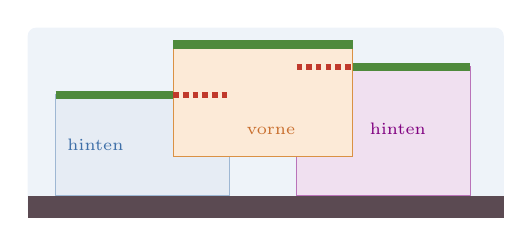
\begin{tikzpicture}[x=1.012pt, y=-1.012pt]
  \fill[sysfill, rounded corners=3pt] (0,6) rectangle (170,74);
  \fill[dock] (0,66) rectangle (170,74);
  \filldraw[fill=violet!12, draw=violet!55] (96,20) rectangle (158,66);
  \filldraw[fill=blue!13, draw=blue!50] (10,30) rectangle (72,66);
  \filldraw[fill=orange!22, draw=orange!90!black] (52,12) rectangle (116,52);
  \draw[green, line width=3pt] (52,12) -- (116,12);
  \draw[green, line width=3pt] (10,30) -- (52,30);
  \draw[green, line width=3pt] (116,20) -- (158,20);
  \draw[red, line width=2pt, dash pattern=on 2pt off 1.5pt] (52,30) -- (72,30);
  \draw[red, line width=2pt, dash pattern=on 2pt off 1.5pt] (96,20) -- (116,20);
  \node[anchor=base west, inner sep=0, font=\fontsize{5.6pt}{6pt}\selectfont, text=orangedark] at (78,44) {vorne};
  \node[anchor=base west, inner sep=0, font=\fontsize{5.6pt}{6pt}\selectfont, text=blue] at (14,50) {hinten};
  \node[anchor=base west, inner sep=0, font=\fontsize{5.6pt}{6pt}\selectfont, text=violet] at (122,44) {hinten};
\end{tikzpicture}

\code{CGWindowListCopyWindowInfo} liefert alle Fenster \textbf{von vorne nach hinten} (nur Positionen, keine Titel \arr\ keine Sonderrechte). Von jeder Oberkante wird abgezogen, was weiter vorne liegt ({\color{red}rot}); der Rest ist begehbar ({\color{green}grün}, \code{Perch}). Volle Bildschirmhöhe = Vollbild/Split View \arr\ kein Klettern. Fenster bewegt \arr\ sie fährt mit; Fenster weg \arr\ sie fällt.

\end{minipage}%
\hspace{11pt}%
%-------------------------------- Spalte 3
\begin{minipage}[t]{189pt}
\sect{Verhalten: der Zustandsautomat}
Immer genau \textbf{eine Phase} (25 insgesamt); ist sie vorbei, entscheidet \code{CatBrain} neu.

\vspace{1pt}
\renewcommand\arraystretch{1.25}
\begin{tabularx}{\linewidth}{@{}>{\bfseries\fontsize{6.4pt}{8pt}\selectfont}p{34pt}@{}X@{}}
Alltag & \tagx{standing}\tagx{walking}\tagx{sittingDown}\tagx{lyingDown}\tagx{sleeping}\tagx{wakingUp}\\
Pflege & \tagx{stretching}\tagx{yawning}\tagx{grooming}\tagx{headWashing}\tagx{backRolling}\tagx{wriggling}\tagx{slowBlinking}\\
Menschen & \tagx[tagin]{petted}\tagx[tagin]{startled}\tagx[tagin]{fleeing}\tagx[tagin]{eating}\tagx[tagin]{chasing}\tagx[tagin]{batting}\tagx[tagin]{watching}\\
Klettern & \tagx[tagcl]{climbingUp}\tagx[tagcl]{climbingDown}\tagx[tagcl]{jumping}\tagx[tagcl]{falling}\\
Streifzug & \tagx[tagro]{away}\\
\end{tabularx}

\vspace{3pt}{\bfseries\fontsize{6.9pt}{9pt}\selectfont Was als Nächstes? – geprüft in dieser Reihenfolge}
\begin{order}
  \item Streifzug ohne Pausenbesuch \arr\ aus dem Bild laufen
  \item Fokus (Pomodoro/Timer) \arr\ hinlegen, fest schlafen
  \item Auf dem Fenster, aber unten gebraucht \arr\ herunter
  \item Timer abgelaufen \arr\ in der Mitte um Aufmerksamkeit werben
  \item Napf voll \arr\ fressen · Pause \arr\ Mitte, strecken, miauen
  \item Knäuel da \arr\ jagen · Runden übrig \arr\ laufen/klettern
  \item sonst \arr\ hinsetzen, hinlegen, schlafen
\end{order}
\callout{\textbf{Temperament} nach Uhrzeit: tags viele Runden, kurze Nickerchen; nachts langer Schlaf. \textbf{Modi}: \code{normal} · \code{focus} · \code{focusBreak}}

\vspace{4pt}
\sect{Grafik: Pixel aus Buchstaben}
\begin{minipage}[c]{54pt}
{\setlength\fboxsep{3.5pt}\colorbox{ink}{\ttfamily\fontsize{5.8pt}{6.6pt}\selectfont
\begin{tabular}{@{}l@{}}
\color{arrow}.K....K.\\
\color{arrow}K\textcolor{orange!60!pink}{P}KKKK\textcolor{orange!60!pink}{P}K\\
\color{arrow}K\textcolor{orange}{O}\textcolor{green!70!white}{E}\textcolor{orange}{OO}\textcolor{green!70!white}{E}\textcolor{orange}{O}K\\
\color{arrow}K\textcolor{orange}{O}\textcolor{green!70!white}{E}\textcolor{orange}{OO}\textcolor{green!70!white}{E}\textcolor{orange}{O}K\\
\color{arrow}K\textcolor{orange}{OW}\textcolor{orange!60!pink}{PP}\textcolor{orange}{WO}K
\end{tabular}}}
\end{minipage}%
\hspace{2pt}{\color{muted}\arr}\hspace{3pt}%
\begin{minipage}[c]{121pt}
Jede Pose ist ein Textraster, ein Buchstabe pro Pixel (\code{K} Umriss, \code{O} Fell, \code{E} Augen). \code{Coat} gibt jedem Buchstaben die Farbe. Augen zu, Spiegeln und Drehen werden \textbf{errechnet}; gemalt wird ohne Glättung.
\end{minipage}

\vspace{5pt}
{\fontsize{5.8pt}{7pt}\selectfont\color{muted}%
\setlength\tabcolsep{4pt}%
\begin{tabular}{@{}ccc@{}}

\includegraphics[height=22pt]{img/walk.png} & 
\includegraphics[height=30pt]{img/sit.png} & 
\includegraphics[height=22pt]{img/stretch.png}\\
laufen & sitzen & strecken
\end{tabular}\\[3pt]
\begin{tabular}{@{}cccc@{}}

\includegraphics[height=15pt]{img/roll.png} & 
\includegraphics[height=30pt]{img/climb.png} &
\shortstack{
\includegraphics[height=19pt]{img/eat.png}\\[-1pt]
\includegraphics[height=8pt]{img/bowl.png}} &

\includegraphics[height=12pt]{img/yarn.png}\\
rekeln & klettern & fressen & Knäuel
\end{tabular}}
\end{minipage}}%
\noindent\usebox\spalten

\end{document}
